% ============================================================================
% Physics (Economics)-Informed Neural Networks (PINNs)
% Summer School on AI for Economics and Finance
% University of Padova, 23-24 September 2026
% Duration: 90 minutes
% ============================================================================

\documentclass[aspectratio=169,11pt]{beamer}

% ---------- Theme and colors ----------
\usecolortheme{dove}
\setbeamertemplate{navigation symbols}{}
\setbeamertemplate{footline}{%
  \hfill\usebeamerfont{page number in head/foot}%
  \usebeamercolor[fg]{normal text}%
  \insertframenumber\,/\,\inserttotalframenumber\kern1em\vskip4pt}
\setbeamerfont{frametitle}{size=\huge}

% ---------- Packages ----------
\usepackage[utf8]{inputenc}
\usepackage[T1]{fontenc}
\usepackage{amsmath,amssymb,amsfonts}
\usepackage{bm}
\usepackage{graphicx}
\usepackage{tikz}
\usetikzlibrary{shapes,arrows.meta,positioning,calc,fit,backgrounds,patterns,decorations.pathreplacing}
\usepackage{pgfplots}
\pgfplotsset{compat=1.18}
% --- readable-from-the-back defaults for every plot ---
\pgfplotsset{every axis/.append style={
    tick label style={font=\footnotesize},
    label style={font=\small},
    title style={font=\small},
    legend style={font=\footnotesize}}}
\usepgfplotslibrary{fillbetween}
\usepackage{booktabs}
\usepackage{hyperref}
\usepackage{multicol}
\usepackage{xcolor}
\usepackage{algorithm}
\usepackage{algorithmic}
\usepackage{array}
\usepackage{listings}

% ---------- Tighter display math, applied uniformly at every font size ------
% (a global typographic setting, so that no frame needs a local \vspace hack)
\makeatletter
\g@addto@macro\normalsize{%
  \setlength\abovedisplayskip{5pt plus 2pt minus 2pt}%
  \setlength\belowdisplayskip{5pt plus 2pt minus 2pt}%
  \setlength\abovedisplayshortskip{2pt plus 1pt}%
  \setlength\belowdisplayshortskip{3pt plus 1pt}}
\g@addto@macro\small{%
  \setlength\abovedisplayskip{4pt plus 2pt minus 2pt}%
  \setlength\belowdisplayskip{4pt plus 2pt minus 2pt}%
  \setlength\abovedisplayshortskip{2pt plus 1pt}%
  \setlength\belowdisplayshortskip{2pt plus 1pt}}
\g@addto@macro\footnotesize{%
  \setlength\abovedisplayskip{3pt plus 2pt minus 2pt}%
  \setlength\belowdisplayskip{3pt plus 2pt minus 2pt}%
  \setlength\abovedisplayshortskip{1pt plus 1pt}%
  \setlength\belowdisplayshortskip{2pt plus 1pt}}
\makeatother

% ---------- Custom colors ----------
\definecolor{uzhblue}{rgb}{0,0,0.5}
\definecolor{uzhgreylight}{RGB}{236,238,241}
\definecolor{uzhgreydark}{RGB}{81,86,94}
\definecolor{harvardcrimson}{RGB}{153,0,0}
\definecolor{unil@blue}{RGB}{0,140,204}
\definecolor{unil@black}{RGB}{35,31,32}
\definecolor{darkgreen}{RGB}{0,100,0}
\definecolor{darkred}{RGB}{139,0,0}
\definecolor{softblue}{RGB}{70,130,180}
\definecolor{softorange}{RGB}{230,159,0}
\definecolor{softgreen}{RGB}{0,158,115}

% ---------- Listings style for Python ----------
% (defined after the colours it references, so the style is not held together
%  by lstset's deferred token expansion)
\lstset{
    language=Python,
    basicstyle=\small\ttfamily,
    keywordstyle=\color{uzhblue}\bfseries,
    commentstyle=\color{uzhgreydark}\itshape,
    stringstyle=\color{darkgreen},
    showstringspaces=false,
    breaklines=true,
    breakatwhitespace=true,
    columns=fullflexible,
    frame=none,
    xleftmargin=0pt,
    aboveskip=4pt,
    belowskip=4pt,
    escapeinside={(*@}{@*)},
}

% ---------- Set beamer colors ----------
\setbeamercolor{frametitle}{bg=uzhgreylight, fg=uzhblue}
\setbeamercolor{title}{fg=uzhblue}
\setbeamercolor{structure}{fg=uzhblue}
\setbeamercolor{block title}{bg=unil@blue, fg=white}
\setbeamercolor{block body}{bg=uzhgreylight}
\setbeamercolor{block title alerted}{bg=darkred,fg=white}
\setbeamercolor{block body alerted}{bg=red!5}
\setbeamercolor{block title example}{bg=darkgreen,fg=white}
\setbeamercolor{block body example}{bg=green!5}
\setbeamercolor{item}{fg=unil@black}
\setbeamercolor{normal text}{fg=unil@black}

% ---------- Emphasis and hyperlinks ----------
\newcommand{\emphc}[1]{\textcolor{harvardcrimson}{#1}}
\hypersetup{colorlinks,linkcolor=harvardcrimson,urlcolor=harvardcrimson}

% ---------- Math commands ----------
\newcommand{\x}{\bm{x}}
\newcommand{\w}{\bm{w}}
\newcommand{\bb}{\bm{b}}
\newcommand{\z}{\bm{z}}
\newcommand{\W}{\bm{W}}
\newcommand{\X}{\bm{X}}
\renewcommand{\a}{\bm{a}}
\newcommand{\R}{\mathbb{R}}
\newcommand{\E}[1]{\mathbb{E}\!\left[#1\right]}
\DeclareMathOperator*{\argmin}{arg\,min}
\DeclareMathOperator*{\argmax}{arg\,max}

% ---------- Title ----------
\title[PINNs II -- Padova 2026]%
{Deep Learning for Solving Dynamic Models}
\subtitle{Session 9: Economics-informed neural networks, economic and financial applications}
\author{Simon Scheidegger}
\institute[HEC Lausanne]{HEC, University of Lausanne\\[4pt]
{\footnotesize Based on Raissi, Perdikaris \& Karniadakis (2019), \emph{Journal of Computational Physics} 378, 686--707}}
\date{University of Padova\\September 24, 2026}

\begin{document}
% --- Exercise pause badge ---
\newcommand{\exercisepause}{%
  \tikz[baseline=(X.base)]{\node[fill=darkgreen!80!black, text=white,
  rounded corners=2pt, inner sep=3pt, font=\scriptsize\bfseries](X){PAUSE, 5 min};}}


% ============================================================================
% PART 0: TITLE & OUTLINE
% ============================================================================

% --- Slide 1: Title ---
{\setbeamercolor{background canvas}{bg=uzhgreylight}
\begin{frame}
\titlepage
\vspace{-0.6cm}
\begin{center}
\begingroup\sloppy\hbadness=10000
{\scriptsize Further: Sirignano \& Spiliopoulos (2018), Deep Galerkin Method for PDEs in high dimensions.}\\[1pt]
{\scriptsize Al-Aradi, Correia, Naez, Hoshisashi \& Schwab (2018), DGM PDE solver.}
\endgroup
\end{center}
\end{frame}
}

% --- Slide 2: Day 2 at a glance (same frame style as the Day 1 lectures) ---
\begin{frame}{Day 2 at a Glance}
\begin{center}
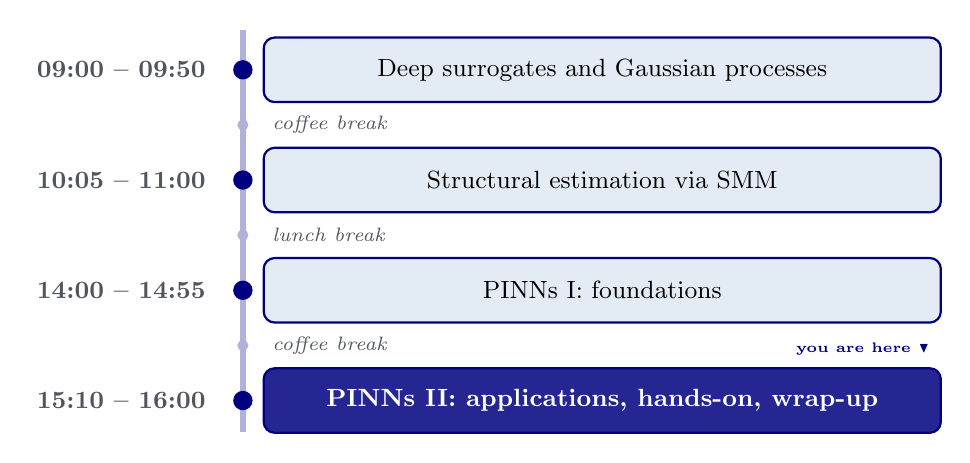
\begin{tikzpicture}[
    session/.style={rectangle, rounded corners=4pt, draw=uzhblue, thick, fill=softblue!15,
                    minimum width=8.6cm, minimum height=0.82cm, align=left, font=\small,
                    inner xsep=10pt, anchor=west},
    now/.style={session, fill=uzhblue!85, draw=uzhblue, text=white, font=\small\bfseries},
    pause/.style={font=\scriptsize\itshape, text=uzhgreydark, anchor=west},
    time/.style={font=\small\bfseries, text=uzhgreydark, anchor=east}
]
    \draw[uzhblue!30, line width=2pt] (0,0.5) -- (0,-4.6);
    \node[time] at (-0.35,0.0) {09:00 -- 09:50};
    \node[session] at (0.25,0.0) {Deep surrogates and Gaussian processes};
    \fill[uzhblue] (0,0.0) circle (3.5pt);
    \node[pause] at (0.25,-0.7) {coffee break};
    \fill[uzhblue!30] (0,-0.7) circle (2pt);
    \node[time] at (-0.35,-1.4) {10:05 -- 11:00};
    \node[session] at (0.25,-1.4) {Structural estimation via SMM};
    \fill[uzhblue] (0,-1.4) circle (3.5pt);
    \node[pause] at (0.25,-2.1) {lunch break};
    \fill[uzhblue!30] (0,-2.1) circle (2pt);
    \node[time] at (-0.35,-2.8) {14:00 -- 14:55};
    \node[session] at (0.25,-2.8) {PINNs I: foundations};
    \fill[uzhblue] (0,-2.8) circle (3.5pt);
    \node[pause] at (0.25,-3.5) {coffee break};
    \fill[uzhblue!30] (0,-3.5) circle (2pt);
    \node[time] at (-0.35,-4.2) {15:10 -- 16:00};
    \node[now] at (0.25,-4.2) {PINNs II: applications, hands-on, wrap-up};
    \fill[uzhblue] (0,-4.2) circle (3.5pt);
    \node[font=\tiny\bfseries, text=uzhblue, anchor=south east] at (8.85,-3.75) {you are here $\blacktriangledown$};
    \end{tikzpicture}
\end{center}
\end{frame}

% --- Slide 3: Outline ---
\begin{frame}{Outline}
\begin{enumerate}
    \item \textbf{From DEQNs to PINNs}\\
    {\small Bridging discrete and continuous time; the PINN loss.}

    \vspace{0.4em}
    \item \textbf{PINN Fundamentals}\\
    {\small Automatic differentiation for PDEs, collocation, training loop.}

    \vspace{0.4em}
    \item \textbf{Soft vs.\ Hard Boundary Conditions}\\
    {\small Trial solutions, 2D Poisson, practical guidance.}

    \vspace{0.4em}
    \item \textbf{Economic Applications: HJB Equation}\\
    {\small Cake-eating problem, scaled trial solution + hard BCs, Adam $\to$ L-BFGS, analytical benchmark; DGM as optional high-D architecture.}

    \vspace{0.4em}
    \item \textbf{Financial Applications: Black--Scholes}\\
    {\small Option pricing via PINNs, comparison with analytical formula.}

    \vspace{0.4em}
    \item \textbf{When to Use One, and What Goes Wrong}\\
    {\small PINNs vs.\ grid solvers, inverse problems, failure modes, and which notebooks to run.}
\end{enumerate}
\end{frame}

% --- Slide 4: Roadmap ---
\begin{frame}{Roadmap of This Session (50 min)}
\textbf{Part II of two.}  Session 8 built the method: a PDE residual on collocation points, and a
deliberate choice between soft and hard boundary conditions.  Now we put it to work.

\vspace{0.6em}
\textbf{IV.\ HJB equations}~~\mbox{\small (14 min)}
\begin{itemize}\setlength\itemsep{1pt}
    \item Cake-eating: scaled trial solution, hard BCs, closed-form benchmark
    \item DGM as an optional high-dimensional architecture
\end{itemize}

\vspace{0.5em}
\textbf{V.\ Finance: Black--Scholes}~~\mbox{\small (6 min)}
\begin{itemize}\setlength\itemsep{1pt}
    \item Option pricing against the closed form; Greeks for free by autodiff
\end{itemize}

\vspace{0.5em}
\textbf{VI.\ When to use one}~~\mbox{\small (10 min)}
\begin{itemize}\setlength\itemsep{1pt}
    \item PINNs vs.\ grid solvers; the other half, inverse problems
    \item Failure modes, and the multi-component loss returning from Session 3
\end{itemize}

\vspace{0.5em}
\textbf{Hands-on}~~\mbox{\small (12 min)}: build a PINN from scratch, at the keyboard.

\vspace{0.3em}
\textbf{Wrap-up}~~\mbox{\small (8 min)}: what to use when, and where to go next.
\end{frame}

% ============================================================================
% PART I: FROM DEQNs TO PINNs
% ============================================================================

% --- Slide 4: Section Divider ---
% --- Padova cut: section 1 "From DEQNs to PINNs" (196 lines) dropped ---
% --- Padova cut: section 2 "PINN Fundamentals" (364 lines) dropped ---
% --- Padova cut: section 3 "Soft vs.\ Hard Boundary Conditions" (473 lines) dropped ---
\section{Economic Applications: the HJB Equation}

\begin{frame}{}
\vfill
\begin{center}
{\Huge \textcolor{uzhblue}{\textbf{Part IV}}}\\[12pt]
{\LARGE Economic Applications: The HJB Equation}
\end{center}
\vfill
\end{frame}

% --- Slide 27: HJB Equation ---
\begin{frame}{The Hamilton--Jacobi--Bellman Equation}
\textbf{Generic continuous-time optimization:}
\[
\rho\, V(\x) = \max_{c}\;\bigl\{u(c) + V_{\x}\cdot f(\x, c)\bigr\}
\]

\vspace{0.3em}
\begin{itemize}
    \item $V(\x)$: \emphc{value function} (unknown)
    \item $\rho$: discount rate
    \item $u(c)$: flow utility
    \item $f(\x,c)$: law of motion for state $\x$
    \item $V_{\x} = \nabla V$: gradient of the value function
\end{itemize}

\vspace{0.4em}
\textbf{This is a PDE!} First-order (or second-order with diffusion).

\vspace{0.3em}
$\Rightarrow$ \emphc{Perfect fit for PINNs:} the network approximates $V$, autograd gives $V_{\x}$, and the HJB residual is the loss.
\end{frame}

% --- Slide 28: Cake-Eating Setup ---
\begin{frame}{Cake-Eating Problem: Setup}
\textbf{A household} with wealth $a(t)$ chooses consumption $c(t)$ to maximize lifetime utility:
\[
\max_{\{c(t)\}} \int_0^\infty e^{-\rho t}\,\frac{c(t)^{1-\gamma}}{1-\gamma}\,\mathrm{d}t
\qquad\text{s.t.}\quad \dot{a} = r\,a - c
\]

\textbf{HJB equation:}\quad
$\rho\,V(a) = \max_c\;\bigl\{\frac{c^{1-\gamma}}{1-\gamma} + V'(a)\,(r\,a - c)\bigr\}$

\vspace{0.2em}
\textbf{FOC:} $c^{-\gamma} = V'(a)$ $\;\Rightarrow\;$ $c^\star = \bigl(V'(a)\bigr)^{-1/\gamma}$.

\vspace{0.2em}
\textbf{Analytical solution} (with $\kappa = \frac{\rho - (1-\gamma)r}{\gamma} > 0$):
\[
V^\star(a) = \frac{\kappa^{-\gamma}}{1-\gamma}\,a^{1-\gamma}, \qquad c^\star(a) = \kappa\,a
\]

{\small Parameters: $\gamma = 2$, $\rho = 0.05$, $r = 0.03$ $\;\Rightarrow\;$ $\kappa = 0.04$.}
\end{frame}

% --- Slide 29: PINN for HJB (trial solution, hard BCs) ---
\begin{frame}{PINN for the HJB Equation: Hard-BC Trial Solution}
\textbf{Anchor + mask + scaled MLP.}  Let $x(a) = (a-a_{\min})/(a_{\max}-a_{\min}) \in [0,1]$ and $S$ a value-scale constant:
\[
\hat V(a) \;=\; V^\star(a_{\min}) + x(a)\bigl[V^\star(a_{\max}) - V^\star(a_{\min})\bigr] \;+\; x(a)\bigl(1-x(a)\bigr)\,S\,f_\theta\bigl(x(a)\bigr).
\]
Endpoints are exact \emph{by construction}, so the boundary loss is identically zero and the optimizer focuses on the HJB residual only.

\vspace{0.3em}
\textbf{Consumption} via FOC, $\hat c(a) = (\hat V'(a))^{-1/\gamma}$, with softplus safeguard on $\hat V'$.

\vspace{0.3em}
\textbf{Loss}: only the interior HJB residual remains,
\[
\ell \;=\; \frac{1}{N}\sum_{i}\mathcal{R}(a_i)^2,
\qquad
\mathcal{R}(a) = \rho\hat V - \Bigl[\tfrac{\hat c^{1-\gamma}}{1-\gamma} + \hat V'(ra - \hat c)\Bigr].
\]

\vspace{0.2em}
{\small \emphc{Pedagogical point:} a small MLP plus hard BCs beats a large gated net with a soft-BC penalty, because the boundary term no longer dominates the objective.}
\end{frame}

% --- Slide 30: DGM Architecture (optional / high-D) ---
\begin{frame}{Optional Architecture for High-D PDEs: DGM}
\begin{columns}[T]
\column{0.44\textwidth}
\begin{center}
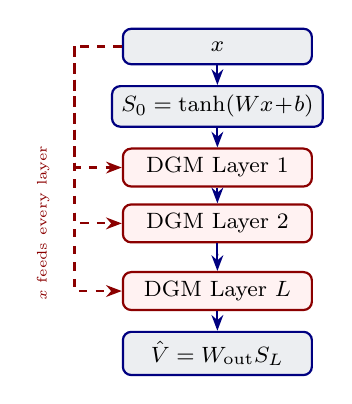
\begin{tikzpicture}[
    block/.style={rectangle, draw=uzhblue, thick, fill=uzhgreylight,
        minimum width=2.4cm, minimum height=0.45cm, font=\footnotesize,
        rounded corners=3pt},
    layer/.style={rectangle, draw=darkred, thick, fill=red!5,
        minimum width=2.4cm, minimum height=0.45cm, font=\footnotesize,
        rounded corners=3pt},
    arr/.style={-{Stealth[length=2mm]}, thick, uzhblue},
    skip/.style={-{Stealth[length=2mm]}, thick, darkred, dashed}
]
    % Input
    \node[block] (inp) {$x$};

    % Initial transform
    \node[block, below=0.25cm of inp] (S0) {$S_0 = \tanh(Wx\!+\!b)$};

    % DGM Layers — stacked to show repetition
    \node[layer, below=0.25cm of S0] (L1) {DGM Layer 1};
    \node[layer, below=0.2cm of L1] (L2) {DGM Layer 2};
    \node[font=\small, text=gray] at ($(L2.south)+(0,-0.18)$) {$\vdots$};
    \node[layer, below=0.35cm of L2] (LL) {DGM Layer $L$};

    % Output
    \node[block, below=0.25cm of LL] (out) {$\hat{V} = W_{\text{out}} S_L$};

    % Vertical arrows
    \draw[arr] (inp) -- (S0);
    \draw[arr] (S0) -- (L1);
    \draw[arr] (L1) -- (L2);
    \draw[arr] (L2) -- (LL);
    \draw[arr] (LL) -- (out);

    % Skip connections from x to every layer
    \draw[skip] (inp.west) -- ++(-0.6,0) |- (L1.west);
    \draw[skip] ([xshift=-0.6cm]inp.west) |- (L2.west);
    \draw[skip] ([xshift=-0.6cm]inp.west) |- (LL.west);

    % Label for skip connections
    \node[font=\tiny, text=darkred, align=center, rotate=90]
        at ([xshift=-1.0cm]L2.west) {$x$ feeds every layer};
\end{tikzpicture}
\end{center}

\column{0.54\textwidth}
\textbf{Deep Galerkin Method}\\
{\small (Sirignano \& Spiliopoulos, 2018)}

\vspace{0.4em}
\begin{itemize}\setlength\itemsep{3pt}
    \item Pays off only in \emphc{higher dimensions}, or where the PDE has sharp features.
    \item The input $x$ enters \emphc{every} layer, not just the first, that is what resolves steep gradients.
    \item Each layer is \emphc{gated}, LSTM-style; the $x$-skips recall Highway Networks.
\end{itemize}

\vspace{0.4em}
\begin{alertblock}{Not the default choice}
\footnotesize
For the 1D cake problem, the trial-solution MLP of the previous slide is simpler \emph{and} more accurate.
\end{alertblock}
\end{columns}
\end{frame}

% --- Slide 31b: Inside a DGM layer ---
\begin{frame}{Inside a DGM Layer}
\begin{columns}[T]
\column{0.56\textwidth}
{\small $S_\ell\in\R^U$ is the depth-$\ell$ hidden state, initialised as $S_0=\tanh(Wx+b)$; $\odot$ is the Hadamard product; and $Z,G,R$ are sigmoid gates valued in $[0,1]$:}
\vspace{0.2em}
{\small\begin{align*}
Z_\ell &= \sigma(U^z x + W^z S_\ell + b^z)\\
G_\ell &= \sigma(U^g x + W^g S_\ell + b^g)\\
R_\ell &= \sigma(U^r x + W^r S_\ell + b^r)\\
H_\ell &= \tanh(U^h x + W^h (S_\ell \odot R_\ell) + b^h)\\
S_{\ell+1} &= (1 - G_\ell)\odot H_\ell + Z_\ell \odot S_\ell
\end{align*}}

\column{0.42\textwidth}
\begin{block}{Reading the gates}
\footnotesize
$R_\ell$ decides how much of the current state enters the candidate $H_\ell$.\\[4pt]
$G_\ell$ and $Z_\ell$ then blend that candidate against the state being carried forward.\\[4pt]
Every one of them sees $x$ directly.
\end{block}

\vspace{0.4em}
{\footnotesize \textbf{Cost:} four weight matrices per layer instead of one, so roughly $4\times$ the parameters of a plain MLP of the same width.}
\end{columns}
\end{frame}

% --- Slide 31: DGM Code ---
\begin{frame}[fragile]{DGM Implementation (PyTorch)}
\begin{lstlisting}[basicstyle=\scriptsize\ttfamily]
class DGMNet(nn.Module):
    def __init__(self, dim, layers=4, units=64):
        super().__init__()
        self.input = nn.Linear(dim, units)
        self.z  = nn.ModuleList(nn.Linear(dim, units) for _ in range(layers))
        self.wz = nn.ModuleList(nn.Linear(units, units) for _ in range(layers))
        # ... similar for g, r, h gates
        self.out = nn.Linear(units, 1)

    def forward(self, x):
        s = torch.tanh(self.input(x))
        for l in range(len(self.z)):
            z = torch.sigmoid(self.z[l](x) + self.wz[l](s))
            g = torch.sigmoid(self.g[l](x) + self.wg[l](s))
            r = torch.sigmoid(self.r[l](x) + self.wr[l](s))
            h = torch.tanh(self.h[l](x) + self.wh[l](s * r))
            s = (1 - g) * h + z * s
        return self.out(s)
\end{lstlisting}
\end{frame}

% --- Slide 32: HJB Residual Code ---
\begin{frame}[fragile]{HJB Residual Implementation}
\begin{lstlisting}[basicstyle=\footnotesize\ttfamily]
def pde_residual(model, a):
    a.requires_grad_(True)
    V = model(a)                        # value function
    V_a = torch.autograd.grad(          # V'(a) via autograd
        V.sum(), a, create_graph=True)[0].squeeze(-1)

    safe_Va = F.softplus(V_a) + 1e-6   # positivity guard
    c = safe_Va.pow(-1.0 / gamma)       # FOC: optimal c
    u_c = c.pow(1-gamma) / (1-gamma)    # flow utility

    R = rho*V - (u_c + safe_Va*(r*a.squeeze(-1) - c))
    return R                            # HJB residual
\end{lstlisting}

\vspace{0.1em}
{\footnotesize The \texttt{softplus} safeguard prevents $V'(a)^{-1/\gamma}$ from blowing up if $V'(a) \leq 0$ during early training.}
\end{frame}

% --- Slide 33: Cake-Eating Results ---
\begin{frame}{Cake-Eating: the Closed-Form Benchmark}
\begin{columns}[T]
\column{0.48\textwidth}
\begin{center}
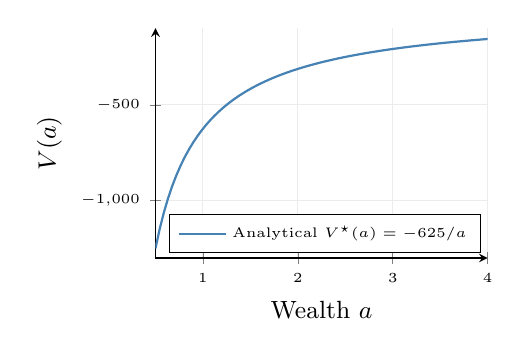
\begin{tikzpicture}
\begin{axis}[
    width=5.8cm, height=4.5cm,
    xlabel={Wealth $a$}, ylabel={$V(a)$},
    xlabel style={font=\small}, ylabel style={font=\small},
    tick label style={font=\tiny},
    xmin=0.5, xmax=4, ymin=-1300, ymax=-100,
    grid=major, grid style={gray!15},
    legend style={font=\tiny, at={(0.98,0.02)}, anchor=south east},
    axis lines=left,
]
    \addplot[thick, softblue, domain=0.5:4, samples=80] {-625/x};
    \addlegendentry{Analytical $V^\star(a) = -625/a$}
\end{axis}
\end{tikzpicture}\\
{\small Value function $V(a)$ (closed form)}
\end{center}

\column{0.48\textwidth}
\begin{center}
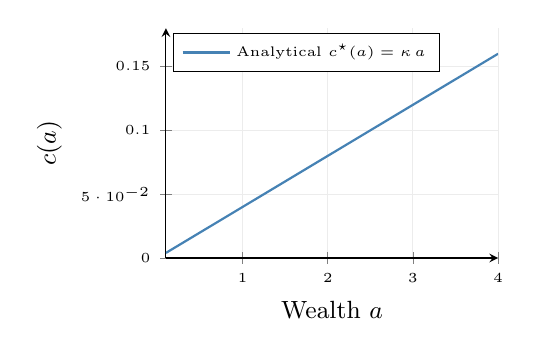
\begin{tikzpicture}
\begin{axis}[
    width=5.8cm, height=4.5cm,
    xlabel={Wealth $a$}, ylabel={$c(a)$},
    xlabel style={font=\small}, ylabel style={font=\small},
    tick label style={font=\tiny},
    xmin=0.1, xmax=4, ymin=0, ymax=0.18,
    grid=major, grid style={gray!15},
    legend style={font=\tiny, at={(0.02,0.98)}, anchor=north west},
    axis lines=left,
]
    \addplot[thick, softblue, domain=0.1:4, samples=80] {0.04*x};
    \addlegendentry{Analytical $c^\star(a) = \kappa\, a$}
\end{axis}
\end{tikzpicture}\\
{\small Consumption policy $c(a)$ (closed form)}
\end{center}
\end{columns}

\vspace{0.1em}
\begin{center}
{\footnotesize These are the \emph{exact} solutions, the target the PINN is scored against. Classroom run: HJB loss $\approx 3\!\times\!10^{-4}$, consumption relative $L^2$ error $\approx 6\!\times\!10^{-3}$. The notebook overlays the fitted $\hat V$ and $\hat c$.}
\end{center}

{\small\hfill\textbf{Notebook:} \texttt{04\_Cake\_Eating\_HJB\_PINN}}
\end{frame}

% --- Slide 34: Extensions ---
\begin{frame}{Extensions: From Cake-Eating to Frontier Models}
\textbf{The PINN/DGM framework scales naturally:}

\vspace{0.3em}
\begin{enumerate}
    \item \textbf{Income risk:} add diffusion $\mathrm{d}a = (ra - c + y)\,\mathrm{d}t + \sigma\,\mathrm{d}W$
    \quad$\Rightarrow$ second-order HJB

    \vspace{0.2em}
    \item \textbf{Aiyagari-type models:} HJB + Kolmogorov Forward Equation
    \quad$\Rightarrow$ coupled PDE system

    \vspace{0.2em}
    \item \textbf{General equilibrium:} prices clear markets
    \quad$\Rightarrow$ hybrid DEQN + PINN

    \vspace{0.2em}
    \item \textbf{High dimensions:} multiple assets, heterogeneous agents
    \quad$\Rightarrow$ no grid needed!
\end{enumerate}

\vspace{0.3em}
{\small See: Achdou et al.\ (2022), Fernandez-Villaverde et al.\ (2024), Gopalakrishna (2024).}
\end{frame}

% ============================================================================
% PART V: BLACK-SCHOLES
% ============================================================================

% --- Slide 35: Section Divider ---
\section{Financial Applications: Black--Scholes}

\begin{frame}{}
\vfill
\begin{center}
{\Huge \textcolor{uzhblue}{\textbf{Part V}}}\\[12pt]
{\LARGE Financial Applications: Black--Scholes}
\end{center}
\vfill
\end{frame}

% --- Slide 36: Black-Scholes PDE ---
\begin{frame}{The Black--Scholes PDE}
\begin{columns}[T]
\column{0.52\textwidth}
\textbf{European call option} ($S$: asset, $K$: strike, $T$: maturity):
\[
\frac{\partial V}{\partial t} + \frac{1}{2}\sigma^2 S^2 \frac{\partial^2 V}{\partial S^2}
+ r S\frac{\partial V}{\partial S} - rV = 0
\]

\textbf{Terminal:} $V(S, T) = \max(S - K, 0)$

\textbf{Boundary conditions:}
\begin{itemize}\setlength{\itemsep}{1pt}
    \item $V(0, t) = 0$
    \item $V(S_{\max}, t) = S_{\max} - Ke^{-r(T-t)}$
\end{itemize}

\column{0.45\textwidth}
\textbf{PINN approach:}
\begin{itemize}\setlength{\itemsep}{2pt}
    \item Network $\mathcal{N}_\theta(S, t) \approx V(S, t)$
    \item Autograd: $V_t$, $V_S$, $V_{SS}$
    \item 4 loss terms:
\end{itemize}

\vspace{0.2em}
{\small
\begin{tabular}{rl}
$\ell_{\text{PDE}}$ & interior residual\\
$\ell_{\text{BC}_0}$ & $V(0,t) = 0$\\
$\ell_{\text{term}}$ & $V(S,T) = \text{payoff}$\\
$\ell_{\text{BC}_{S_{\max}}}$ & far-field BC\\
\end{tabular}
}
\end{columns}
\end{frame}

% --- Slide 37: Black-Scholes Implementation ---
\begin{frame}[fragile]{Black--Scholes PINN: Key Code}
\begin{lstlisting}
def pde_residual(model, S, t):
    S.requires_grad_(True)
    t.requires_grad_(True)
    X = torch.cat([S, t], dim=1)
    V = model(X)

    V_t  = torch.autograd.grad(V, t, (*@\ldots@*))[0]
    V_S  = torch.autograd.grad(V, S, (*@\ldots@*))[0]
    V_SS = torch.autograd.grad(V_S, S, (*@\ldots@*))[0]

    # Black-Scholes PDE residual
    res = V_t + 0.5*sigma**2*S**2*V_SS + r*S*V_S - r*V
    return res
\end{lstlisting}

\vspace{0.1em}
{\small\textbf{Loss:}
\[
\ell = \text{MSE}(\text{res}) + \text{MSE}(V|_{S=0}) + \text{MSE}(V|_{t=T} - \text{payoff}) + \text{MSE}(V|_{S_{\max}} - \text{target})
\]
}
\end{frame}

% --- Slide 38: Black-Scholes Results ---
\begin{frame}{Black--Scholes: the Closed-Form Benchmark}
\begin{columns}[T]
\column{0.55\textwidth}
\begin{center}
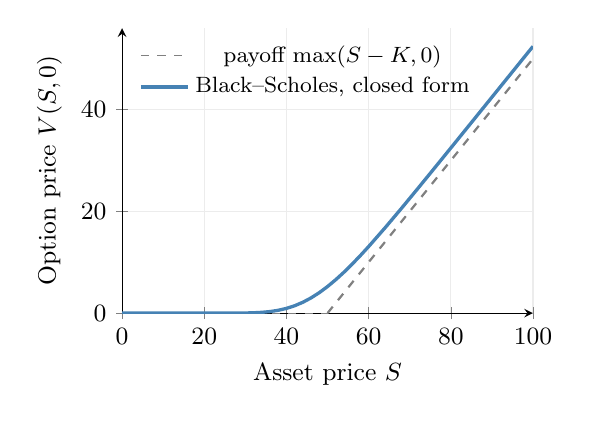
\begin{tikzpicture}
\begin{axis}[
    width=6.8cm, height=5.2cm,
    xlabel={Asset price $S$}, ylabel={Option price $V(S, 0)$},
    xlabel style={font=\small}, ylabel style={font=\small},
    tick label style={font=\small},
    xmin=0, xmax=100, ymin=0, ymax=56,
    grid=major, grid style={gray!15},
    legend style={font=\footnotesize, at={(0.02,0.98)}, anchor=north west, draw=none, fill=none},
    axis lines=left,
]
    \addplot[thick, gray, dashed, domain=0:100, samples=2, forget plot] coordinates {(50,0) (100,50)};
    \addplot[gray, dashed, domain=0:50, samples=2] coordinates {(0,0) (50,0)};
    \addlegendentry{payoff $\max(S-K,0)$}
    \addplot[very thick, softblue] coordinates {
      (0,0.000) (10,0.000) (20,0.000) (24,0.001) (26,0.002) (28,0.009)
      (30,0.027) (32,0.069) (34,0.154) (36,0.307) (38,0.556) (40,0.930)
      (42,1.451) (44,2.138) (46,2.997) (48,4.029) (50,5.225) (52,6.571)
      (54,8.049) (56,9.640) (58,11.324) (60,13.085) (64,16.772) (68,20.605)
      (72,24.520) (76,28.477) (80,32.457) (86,38.444) (92,44.440) (100,52.439)};
    \addlegendentry{Black--Scholes, closed form}
\end{axis}
\end{tikzpicture}
\end{center}

\column{0.42\textwidth}
{\small
\textbf{Parameters:} $K = 50$, $T = 1$, $r = 0.05$, $\sigma = 0.2$, $S_{\max} = 100$.

\vspace{0.2em}
\textbf{Network:} 3 hidden layers, 64 units, $\tanh$; 2{,}500 Adam epochs, then 300 L-BFGS iterations.

\vspace{0.3em}
The gap between the curves is the \emphc{time value}: at the money the option is worth $5.23$, not $0$.

\vspace{0.3em}
Against this benchmark the notebook reports max absolute error $\approx 0.13$, mean $\approx 0.04$, and plots the PINN overlay.
}
\end{columns}

\vspace{0.2em}
{\small\hfill\textbf{Notebook:} \texttt{05\_Black\_Scholes\_PINN}}
\end{frame}

% ============================================================================
% PART VI: PATHOLOGIES, HANDS-ON, AND WRAP-UP
% ============================================================================

\section{When to Use One, and What Goes Wrong}

% --- Slide 38b: Section Divider ---
\begin{frame}{}
\vfill
\begin{center}
{\Huge \textcolor{uzhblue}{\textbf{Part VI}}}\\[12pt]
{\LARGE When to Use One, and What Goes Wrong}
\end{center}
\vfill
\end{frame}

% --- Slide 38b2: Honest comparison against a classical solver ---
\begin{frame}{Should You Use a PINN at All?}
\textbf{On a 1D problem, finite differences win. Outright.}

\vspace{0.4em}
\begin{columns}[T]
\column{0.52\textwidth}
{\small Notebook \texttt{07} solves the same partial-equilibrium HJB both ways:}
\begin{itemize}\setlength\itemsep{2pt}
    \item \emphc{Upwind implicit FD}: 13 iterations on a 500-point grid, then the error is whatever the discretization gives you, and you can shrink it by refining.
    \item \emphc{PINN}: thousands of epochs to reach $10^{-3}$--$10^{-2}$, with no comparable knob.
\end{itemize}

\vspace{0.5em}
{\small Anyone selling you PINNs as a universal replacement for a grid solver is overselling.}

\vspace{0.3em}

\column{0.45\textwidth}
\begin{block}{Where the trade flips}
\footnotesize
A tensor grid needs $n^d$ points. At $n=50$:\\[3pt]
\begin{tabular}{@{}rl@{}}
$d=1$ & $50$ \\
$d=2$ & $2{,}500$ \\
$d=4$ & $6.3$ million \\
$d=6$ & $1.6\times10^{10}$ \\
\end{tabular}\\[4pt]
Collocation cost is set by the \emph{sample size you choose}, not by $d$.
\end{block}
\end{columns}

\vspace{0.4em}
{\footnotesize \emphc{Use a PINN when} the state space is high-dimensional, the domain is irregular, there are many discrete states, or you need the solution \emph{and} its derivatives as a differentiable object. Otherwise, use the grid.}
\end{frame}

% --- Slide 38b3: The other half of Raissi et al. ---
\begin{frame}{The Other Half: Inverse Problems}
\textbf{So far the PDE was known and we solved it.} Raissi et al.\ (2019) also treat the reverse.

\vspace{0.4em}
\begin{columns}[T]
\column{0.48\textwidth}
\begin{block}{Forward problem}
\small
Parameters $\mu$ given, solve for $u$.\\[4pt]
$\ell(\theta) = \|\mathcal{D}_\mu[\mathcal{N}_\theta]\|^2 + \text{BCs}$
\end{block}

\column{0.48\textwidth}
\begin{alertblock}{Inverse problem}
\small
Some data on $u$ observed, solve for $u$ \emph{and} $\mu$.\\[4pt]
$\ell(\theta,\mu) = \|\mathcal{D}_\mu[\mathcal{N}_\theta]\|^2 + \|\mathcal{N}_\theta - u^{\text{obs}}\|^2$
\end{alertblock}
\end{columns}

\vspace{0.5em}
\begin{itemize}\setlength\itemsep{3pt}
    \item $\mu$ is just \emphc{another set of trainable parameters}: one extra tensor, same optimizer, same loop.
    \item In economics $\mu$ is a \emphc{structural parameter}, risk aversion, a discount rate, an adjustment cost, and the data term is a moment condition.
    \item This is estimation and solution in \emphc{one} optimization, rather than a solver nested inside an estimation loop.
\end{itemize}

\vspace{0.3em}
{\footnotesize Connects directly to the deep-surrogate approach to structural estimation from Day 1.}
\end{frame}

% --- Slide 38c: When PINNs fail — the multi-component loss again ---
\begin{frame}{When PINNs Fail: the Multi-Component Loss, Again}
\textbf{The soft-BC loss is a weighted sum of residuals that live at different scales:}
\[
\ell_\theta = \underbrace{\lambda_{\text{pde}}\,\ell_{\text{pde}}}_{\text{interior}}
\;+\; \underbrace{\lambda_{\text{bc}}\,\ell_{\text{bc}}}_{\text{boundary}}
\;+\; \underbrace{\lambda_{\text{ic}}\,\ell_{\text{ic}}}_{\text{initial}}
\]

\vspace{0.5em}
\begin{columns}[T]
\column{0.50\textwidth}
\textbf{This is exactly the Day 1 pathology.}
\begin{itemize}\setlength\itemsep{2pt}
    \item A residual carrying $S^2\partial_{SS}V$ is not in the same units as one carrying $V$ itself.
    \item The largest-scale component captures the gradient; the others are effectively ignored.
    \item Adaptive weights cannot close a gap of several orders of magnitude.
\end{itemize}

\column{0.47\textwidth}
\begin{block}{What to do, in order}
\small
\textbf{1.}~\emphc{Non-dimensionalize} first, rescale so every residual is $O(1)$.\\[3pt]
\textbf{2.}~Enforce \emphc{structurally} where you can: a hard-BC trial solution deletes $\ell_{\text{bc}}$ from the sum.\\[3pt]
\textbf{3.}~Only then reach for adaptive weights.
\end{block}
\end{columns}

\vspace{0.3em}
{\footnotesize On Day 1 this bought $\approx 110\times$ over equal weighting, where the best adaptive scheme managed $2\times$ (\texttt{02\_DEQN.pdf}, Part IV). See Wang, Teng \& Perdikaris (2021).}
\end{frame}

% --- Slide 38d: Hands-on ---
\begin{frame}{Hands-On: What to Run}
\textbf{All seven notebooks are PyTorch, CPU-only, and self-contained.}\\[2pt]
{\footnotesize Run them on \href{https://nuvolos.cloud}{nuvolos.cloud}, no local setup needed.}

\vspace{0.4em}
\textbf{Session 8, the method}
\begin{itemize}\setlength\itemsep{1pt}
    \item The simplest possible PINN: $y''=-1$ with zero BCs \hfill{\footnotesize\texttt{08\_01}}
    \item Soft penalty vs.\ hard trial solution, the core choice \hfill{\footnotesize\texttt{08\_02}}
    \item 2D Poisson: hard BCs by transfinite interpolation \hfill{\footnotesize\texttt{08\_03}}
\end{itemize}

\vspace{0.3em}
\textbf{Session 9, the applications}
\begin{itemize}\setlength\itemsep{1pt}
    \item The first economic application: the cake-eating HJB \hfill{\footnotesize\texttt{09\_01}}
    \item Black--Scholes, Greeks for free by autodiff \hfill{\footnotesize\texttt{09\_02}}
    \item PE HJB with discrete income, against an FD benchmark \hfill{\footnotesize\texttt{09\_03}}
\end{itemize}

\vspace{0.1em}
\begin{exampleblock}{Now: build one yourself \hfill{\footnotesize\texttt{09\_04}}}
\footnotesize
A fill-in-the-blank PINN for $u''+u=0$ on $[0,\pi]$, solution $\sin(x)$.  We start it together
now; solutions follow each task in the same file, so you can finish it afterwards.
\end{exampleblock}
\end{frame}

% --- Slide 39: Summary ---
\begin{frame}{Summary and Key Takeaways}
\begin{columns}[T]
\column{0.32\textwidth}
\begin{block}{Method}
\centering\small
\vspace{0.2em}
PINNs embed \emphc{differential equations} directly into the neural network loss function via \emphc{automatic differentiation}.
\vspace{0.2em}
\end{block}

\column{0.32\textwidth}
\begin{block}{Boundary Conditions}
\centering\small
\vspace{0.2em}
\emphc{Hard BCs} (trial solutions) eliminate tuning and ensure exact satisfaction. Use \emphc{soft BCs} for complex domains.
\vspace{0.2em}
\end{block}

\column{0.32\textwidth}
\begin{block}{Applications}
\centering\small
\vspace{0.2em}
HJB equations, Black--Scholes, and any continuous-time model. Scales to \emphc{high dimensions} without grids.
\vspace{0.2em}
\end{block}
\end{columns}

\vspace{0.6em}
\textbf{From DEQNs to PINNs:}
\begin{itemize}
    \item \emphc{Same philosophy:} economic/financial equations \emph{are} the loss
    \item \emphc{New ingredient:} \texttt{torch.autograd.grad} for derivatives of $\mathcal{N}_\theta$
    \item \emphc{Broader scope:} any PDE, not just algebraic equilibrium conditions
\end{itemize}
\end{frame}

% --- Slide 40: Questions ---
\begin{frame}{}
\begin{columns}[c]
\column{0.45\textwidth}
\begin{center}
{\Huge \textcolor{uzhblue}{\textbf{Questions?}}}

\vspace{1.0cm}
{\large Simon Scheidegger}\\[4pt]
{\small HEC, University of Lausanne}\\[4pt]
\url{https://sischei.github.io}

\vspace{0.6cm}
{\small Materials:~~\href{https://github.com/sischei/deep_learning_padova_0926}{github.com/sischei/deep\_learning\_padova\_0926}}
\end{center}

\column{0.45\textwidth}
\begin{center}
\textbf{Companion Notebooks:}\\[8pt]
{\small
\begin{tabular}{rl}
01 & ODE PINN (zero BCs) \\
02 & Soft vs.\ hard BCs \\
03 & 2D Poisson \\
04 & Cake-eating HJB \\
05 & Black--Scholes \\
06 & Exercise: build a PINN \\
07 & PE HJB: FD vs.\ PINN \\
\end{tabular}
}

\vspace{0.7cm}
\textbf{Next up:}\\[6pt]
{\large Hands-on, then}\\
{\large the course wrap-up}
\end{center}
\end{columns}
\end{frame}

\end{document}
